\chapter{HASIL DAN PEMBAHASAN} \label{cha:4-HasilDanPembahasan}

\section{Hasil Pemelajaran Model} \label{sec:4-PersiapanPengujian}

Pemelajaran model yang dilakukan selama sepuluh \textit{epochs} menunjukkan bahwa kesalahan model
dalam mengestimasi pose tiga dimensi berkurang dalam setiap \textit{epoch}. \text{Learning rate}
yang dibagi dua dalam setiap \textit{epoch} mempengaruhi pemelajaran model dimana penyesuaian model
semakin teliti. Adaptasi bobot model terjadi secara drastis pada \textit{epoch} 0 sampai dengan
\textit{epoch} 3. \textit{Epoch} 4 dan seterusnya menggunakan \textit{learning rate} yang semakin
kecil sehingga model semakin teliti dalam melakukan adaptasi. Grafik pemelajaran model dapat dilihat
pada gambar~\ref{fig:pelatihan}.

\begin{figure}[htbp]
    \begin{center}
        \fbox{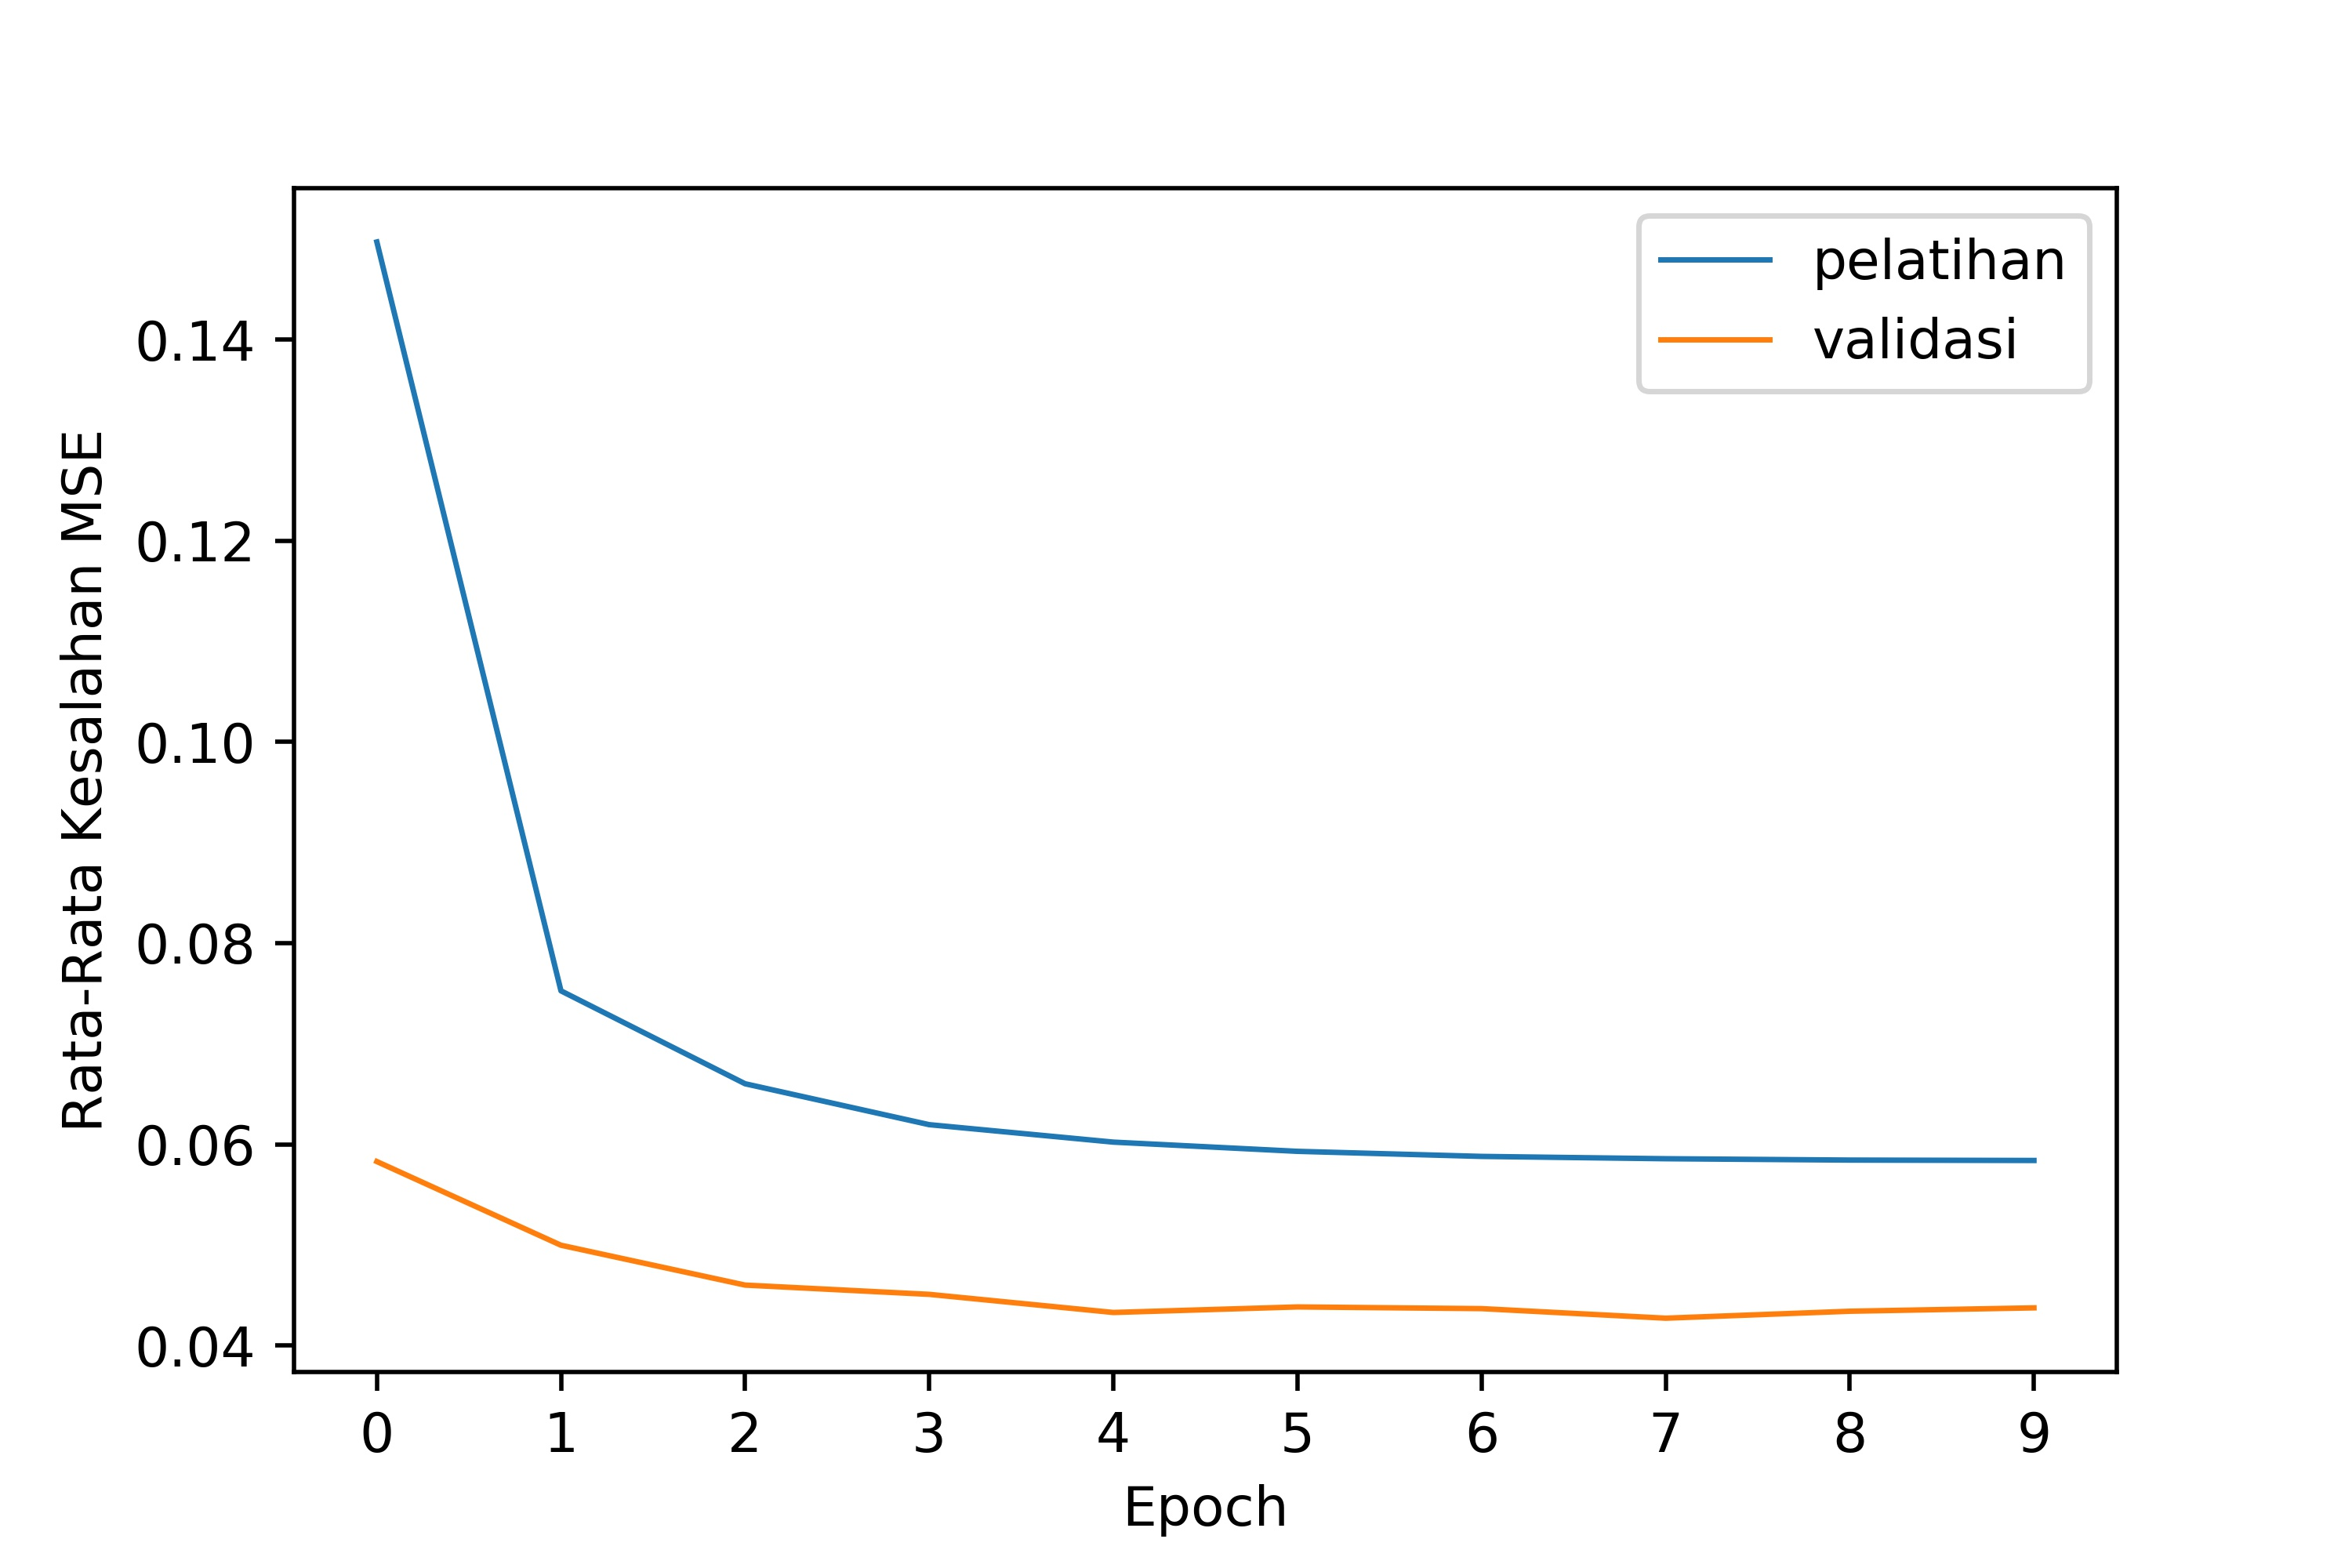
\includegraphics[width=11.9cm]{bab4/gambar/pelatihan.jpg}}
    \end{center}
    \vspace{-20pt}
    \captionsetup{labelfont=bf, textfont=bf}
    \caption{Grafik Pemelajaran Model}
    \vspace{-10pt}
    \captionsetup{labelfont=md, textfont=md}
    % \caption*{Sumber: sumber}
    % \caption*{Sumber: nama(2019)}
    \label{fig:pelatihan}
\end{figure}

\section{Analisis Uji Coba Aplikasi} \label{sec:4-PersiapanPengujian}

Inferensi yang bagus akan terjadi apabila langkah-langkah pada tahapan uji coba tidak mengalami
kesalahan. Kualitas gambar dan pose yang tidak cacat juga mempengaruhi proses dari awal hingga akhir.
Prapemrosesan gambar pada data inferensi yang tepat memudahkan OpenPose dalam mencari titik kunci
pose dua dimensi secara lengkap. Titik kunci OpenPose yang lengkap kemudian memenuhi syarat untuk
dikonversi menjadi spesifikasi yang diinginkan. Informasi tersebut kemudian diteruskan ke model
untuk mendapatkan titik kunci pose tiga dimensi.
% Rangkaian langkah-langkah yang baik menghasilkan
% pose tiga dimensi yang realistis seperti pada gambar~\ref{fig:bro75}.

% \begin{figure}[htbp]
%     \begin{center}
%         \fbox{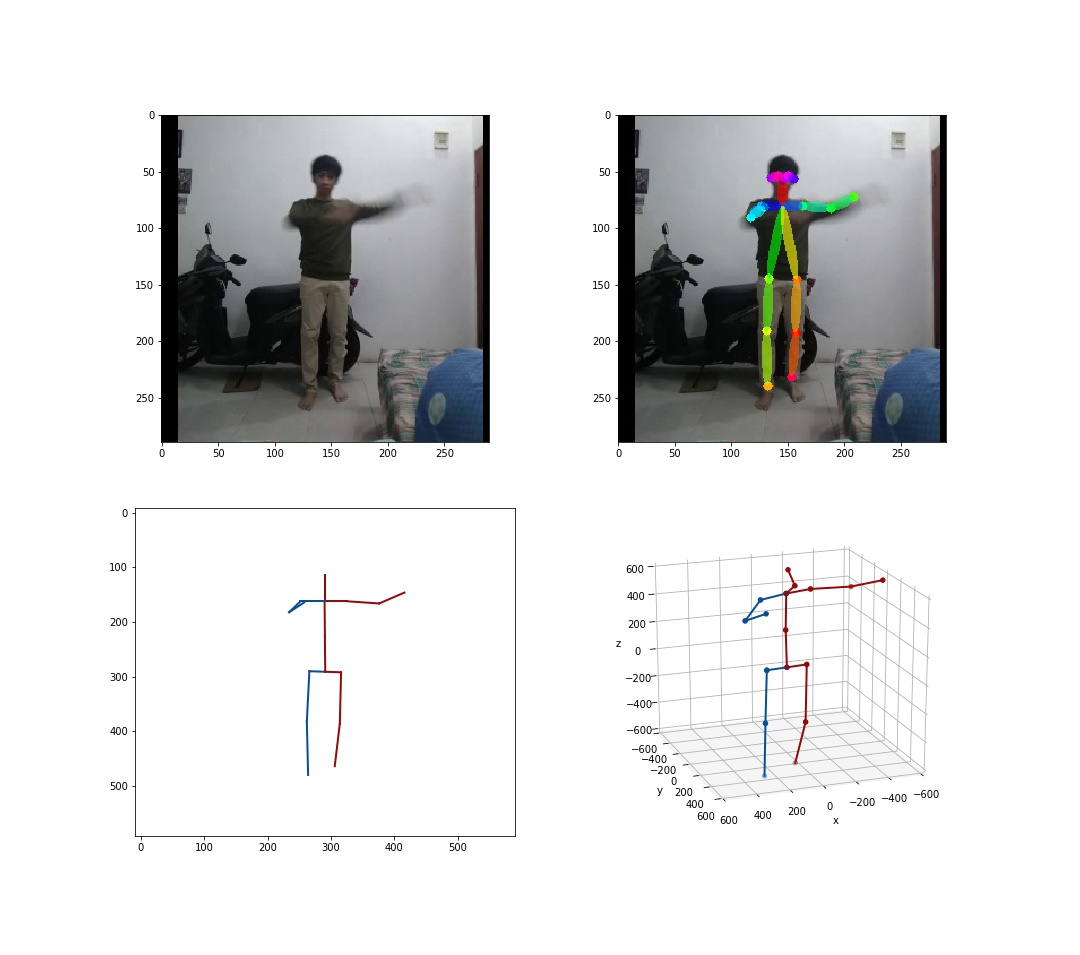
\includegraphics[width=11.9cm]{bab4/gambar/bro75.jpg}}
%     \end{center}
%     \vspace{-20pt}
%     \captionsetup{labelfont=bf, textfont=bf}
%     \caption{Inferensi Tepat}
%     \vspace{-10pt}
%     \captionsetup{labelfont=md, textfont=md}
%     % \caption*{Sumber: sumber}
%     % \caption*{Sumber: nama(2019)}
%     \label{fig:bro75}
% \end{figure}

Kualitas pose yang cacat menghasilkan estimasi pose tiga dimensi yang cacat. Oklusi pose pada gambar
dua dimensi dapat menghilangkan suatu bagian tubuh. Hilangnya bagian ini dari gambar menyebabkan
kesalahan pada langkah-langkah selanjutnya. Titik kunci lengan kanan hilang ketika pose lengan
mengarah lurus ke lensa kamera sehingga terjadi oklusi. Hal ini menyebabkan OpenPose tidak dapat
menemukan titik kunci lengan kanan dan memberi nilai nol pada titik kunci tersebut. Proses konversi
dan inferensi titik kunci tiga dimensi juga menghasilkan pose yang tidak realistis. Inferensi pose
hilang yang diakibatkan oklusi dapat dilihat pada gambar~\ref{fig:bro76}.

\begin{figure}[htbp]
    \begin{center}
        \fbox{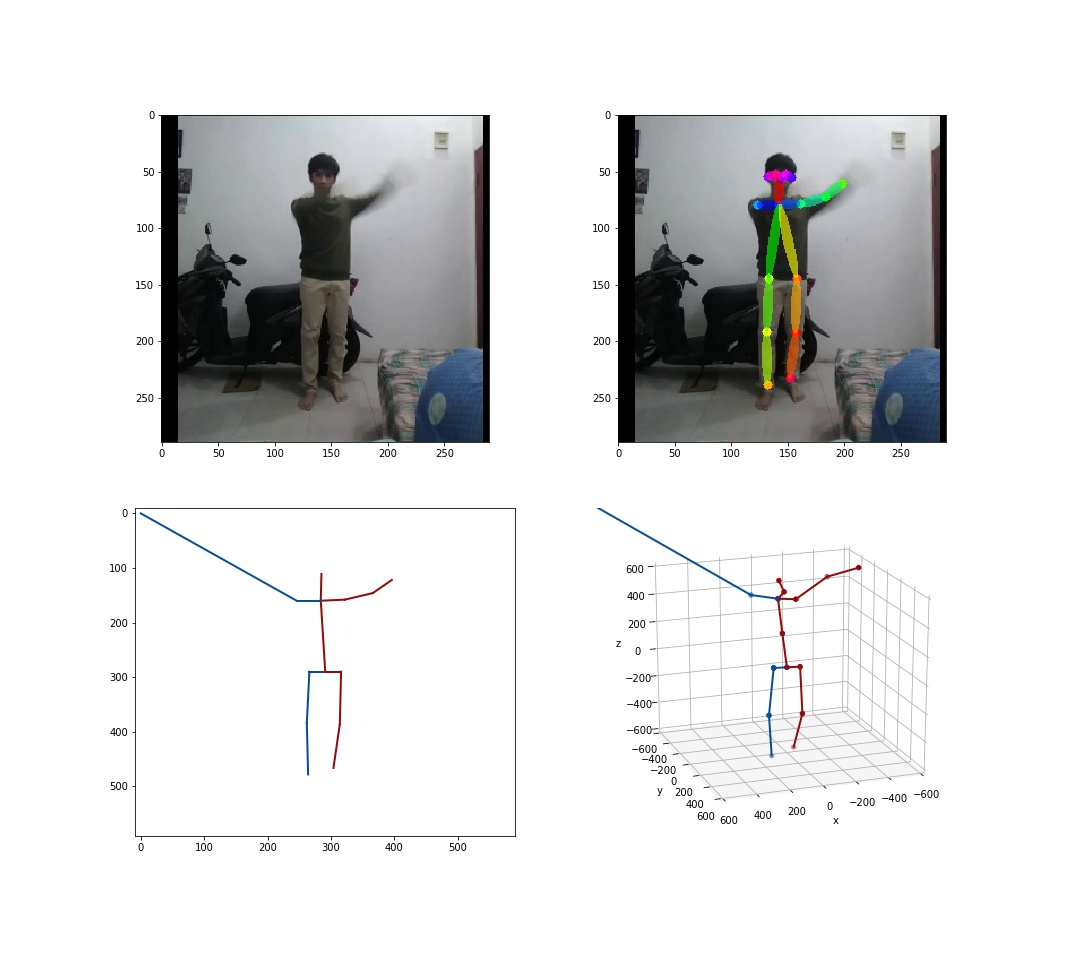
\includegraphics[width=11.9cm]{bab4/gambar/bro76.jpg}}
    \end{center}
    \vspace{-20pt}
    \captionsetup{labelfont=bf, textfont=bf}
    \caption{Inferensi Pose Hilang}
    \vspace{-10pt}
    \captionsetup{labelfont=md, textfont=md}
    % \caption*{Sumber: sumber}
    % \caption*{Sumber: nama(2019)}
    \label{fig:bro76}
\end{figure}

\pagebreak

Kesalahan juga dapat terjadi pada proses inferensi titik kunci. Apabila OpenPose mengeluarkan
\textit{output} yang ambigu dimana terdapat titik kunci yang dianggap sebagai bagian dari tubuh manusia.
OpenPose menghasilkan titik kunci ganda yang tidak sesuai dengan spesifikasi yang diperlukan meskipun
berhasil mendeteksi pose secara lengkap.
Hasil keluaran yang tidak sesuai dengan spesifikasi model mengakibatkan estimasi pose tiga dimensi yang rusak.
Inferensi pose yang mengalami kesalahan deteksi dapat dilihat pada gambar~\ref{fig:bro131}.

\begin{figure}[htbp]
    \begin{center}
        \fbox{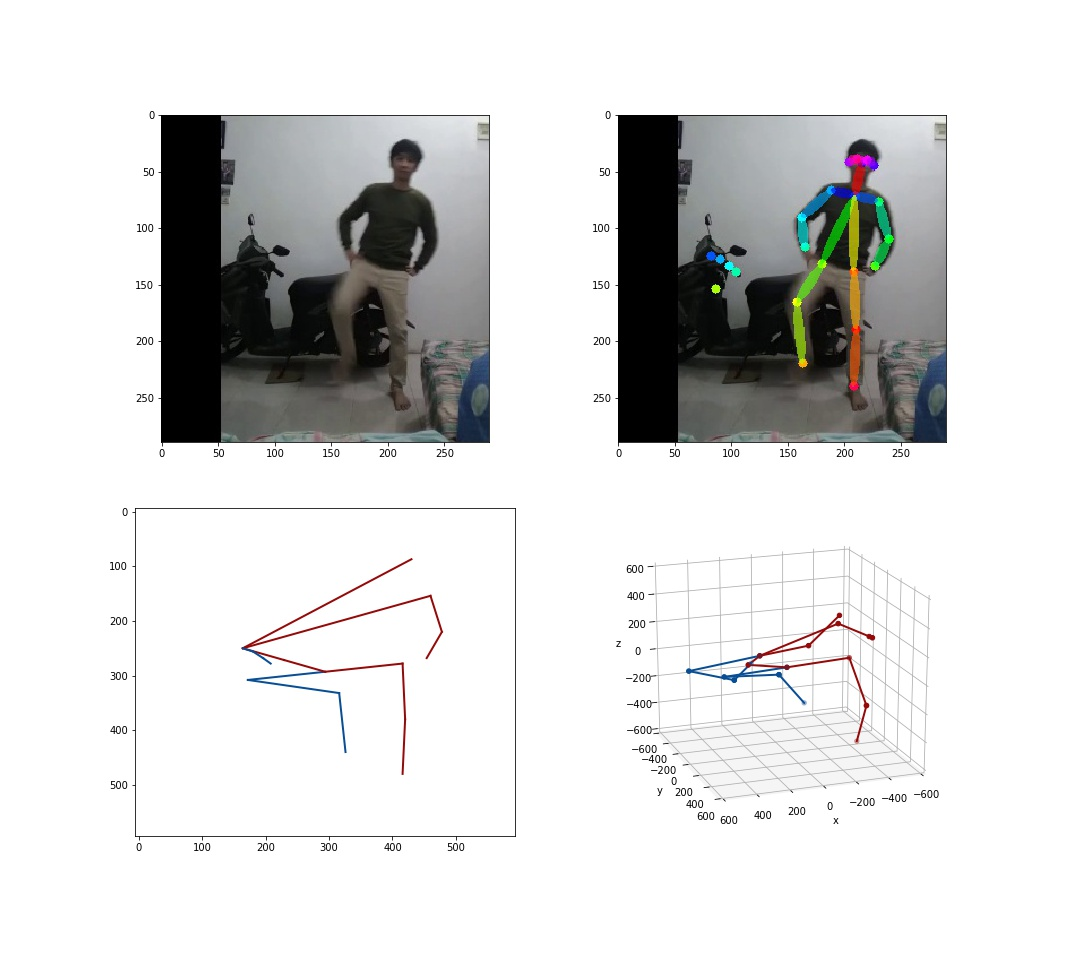
\includegraphics[width=11.9cm]{bab4/gambar/bro131.jpg}}
    \end{center}
    \vspace{-20pt}
    \captionsetup{labelfont=bf, textfont=bf}
    \caption{Kesalahan Deteksi}
    \vspace{-10pt}
    \captionsetup{labelfont=md, textfont=md}
    % \caption*{Sumber: sumber}
    % \caption*{Sumber: nama(2019)}
    \label{fig:bro131}
\end{figure}